% !TEX root = dev-manual.tex
% ERA-Großpraktikum: Entwickleranleitung -- QtCreator stup

\paragraph{Aufsetzen von QtCreator}

QtCreator ist eine integrierte Entwicklungsumgebung, die von Qt selbst zur
Verfügung gestellt wird und somit alle Features von Qt (QML, Widget-Designer
etc.) nativ unterstützt. Da die IDE auch C++-Programmierung unterstützt, eignet
sie sich als Allrounder-IDE für dieses Projekt. Im Folgenden werden das
Aufsetzen von QtCreator und erste Schritte danach für Ubuntu 16.10 beschrieben.

\subparagraph{QtCreator installieren}

QtCreator kann meist über den Paketmanager mit folgendem Befahl installiert werden: \texttt{apt install qtcreator}.

\subparagraph{Repository klonen}

Siehe \autoref{dev-report-cmake-build}. Endet die Ausführung von \texttt{cmake}
in einem Fehler "Could not find a package configuration file provided by
Qt5Widgets", dann ist vermutlich bei der Installation von
\texttt{qtdeclarative5-dev} etwas missglückt.

\subparagraph{QtCreator und CMake}

Im Startbildschirm \texttt{Open Project} und das \texttt{CMakeLists.txt} in der
Wurzel des Projekts öffnen. Im Reiter \texttt{Configure Project} für das Kit
\texttt{Desktop} $\rightarrow$ \texttt{Details}: Nur \texttt{Debug und Release}
anhaken und die Build-Ordner anpassen\footnote{Es bietet sich an, für die IDE
einen anderen Build-Ordner zu verwenden, als für das Bauen über die Konsole. Ein
CMake-Projekt in QtCreator wird mit CodeBlocks erzeugt und erstellt daher leicht
andere Konfigurationsdateien als CMake über die Konsole. Damit beides parallel
nebeneinander betrieben werden kann, sollten die Build-Ordner getrennt werden.}.
Die Auswahl bestätigen. Jetzt sollte das Edit-Tab mit dem Projekt geöffnet sein.
Im unteren Rand unter "General Messages" sollte einmal CMake automatisch
aufgerufen worden sein, links oben im \texttt{Projects} Fenster sollte die
Struktur des Projekts (mit CMakeLists.txt, include, source, tests und
third-party) zu sehen sein. Im Projects-Tab (linker Rand, Schraubenschlüssel) im
Reiter \texttt{Build \& Run} wird jetzt der Build-Prozess konfiguriert. Bei
\texttt{Edit build configuration} Debug auswählen, dann die Einstellungen im
\texttt{Build Steps}-Fenster wie in \autoref{fig:build-run} verändern.

\begin{figure}[h!]
	\centering
	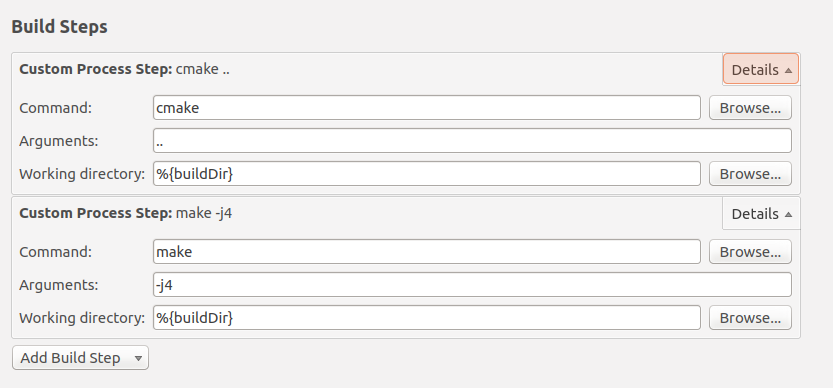
\includegraphics[scale=0.5]{images/setup-qtcreator-buildrun-config.png}
	\caption{Das Build \& Run Konfigurationsfenster in QtCreator.}
  \label{fig:build-run}
\end{figure}

Der Eintrag von \texttt{CMake Arguments} soll dabei der relative Pfad vom
eingetragenen Build-Ordner zum obersten Ordner des Projekts sein. Im Beispiel
ist der Build-Order unter \texttt{era-gp-sim/build\_qtcreator\_debug} angelegt,
d.h. eine Ebene höher liegt der root-Ordner des Projekts. Das \texttt{-j4}
Argument bei \texttt{make} erhöht die Geschwindigkeit beim Bauen, da 4 Jobs
gleichzeitig ausgeführt werden. Im Anschluss zur Run-Konfiguration wechseln
(\autoref{fig:run-config}) und als "Working Directory" den Build-Ordner
eintragen.

\begin{figure}[h!]
	\centering
	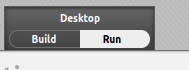
\includegraphics[trim={0 0.4cm 0.8cm 0}, clip]{images/setup-qtcreator-run-config}
	\caption{Zur Run-Konfiguration wechseln}
	\label{fig:run-config}
\end{figure}

Nun zurück wechseln und bei \texttt{Edit build configuration} Release auswählen
und sowohl \texttt{Build Steps} als auch \texttt{Run} wie oben verändern. Ins
Edit-Tab wechseln und am linken Rand unten beim Monitor von \texttt{Release} auf
\texttt{Debug} wechseln und dann mit Klick auf den Hammer das Projekt bauen.

\begin{figure}[h!]
	\centering
	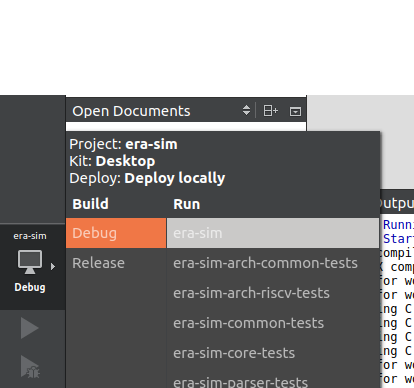
\includegraphics[trim={1.4cm 0cm 0.5cm 2.5cm}, clip, scale=0.7]{images/setup-qtcreator-change-buildrun-flavor.png}
	\caption{Verschiedene Ausführungsoptionen}
\end{figure}

Hier können dann später statt \texttt{era-sim} verschiedene Test-Suites lokal
ausgeführt werden. In der \texttt{Compile Output} Konsole kann der Fortschritt
des Bauvorgangs überwacht werden.

\subparagraph{Nützliche Einstellungen}

QtCreator weist noch viele weitere Features auf, als jene, die hier beschrieben
wurden. Nennenswert sind unter diesen jedoch

\begin{itemize}
  \bolditem{File Naming}: Im Menü \texttt{Tools $\rightarrow$ Options}, dort in der linken Auswahlliste C++ $\rightarrow$
  Reiter \texttt{File Naming}: Bei Headers Suffix zu hpp ändern.

  \bolditem{Lizenz automatisch einfügen}: Im Menü \texttt{Tools $\rightarrow$
  Options $\rightarrow$ C++ $\rightarrow$ FileNaming}: Unter "License Template"
  kann der Pfad zu einer Textdatei eingegeben werden, deren Inhalt dann als
  Kommentar an den Anfang jeder neu erzeugten Datei platziert wird.

  \bolditem{Auto-Formatting}: Muss evtl. über \texttt{Help
  $\rightarrow$ About plugins} heruntergeladen werden (\texttt{Beautifier}). Ist
  dann unter \texttt{Tools $\rightarrow$ Options $\rightarrow$ Beautifier} zu
  finden.
\end{itemize}
